\begin{question}
  \hspace*{\fill} [Note Maximale: ?]\par
  \medskip
  \noindent Indroduction à la question.\par
  \medskip
  \noindent Introduction au diagramme.\par
  \medskip
  \begin{center} % or flushleft or flushright
    \noindent Commentaire au-dessus du diagramme\par
    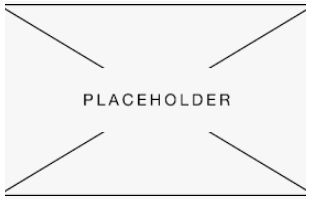
\includegraphics[scale=0.8]{placeholder}\par
    \noindent Commentaire en-dessous du diagramme\par
  \end{center} % or flushleft or flushright

  %% Chose one or the other of these two options
  % Option 1. A single question with no breakdown into parts
  \medskip
  \noindent Un seul bloc de paragraphes qui décrit la question.  La valeure maximale de la note entre parentheses carrées à la marge droite de la derniere ligne.\hspace*{\fill} [?]\par
  
  % Option 2. A question broken down into a list of parts each with its component maximum mark
 
  \noindent OU peut-être quelques elements generals de la question - elements auquels les parties de la question peuvent se reférer - suivis ensuite d'úne question en parties.\par
  \begin{enumerate}[label=(\alph*)]
    \item une partie\hspace*{\fill} [?]
    \item une autre partie
      \begin{enumerate}[label=(\roman*)]
        \item une subdivision de la partie\hspace*{\fill} [?] % optionally omit this mark and let the last sub-item be the sum of the sub-items
        \item une authre sub-division\hspace*{\fill} [?]
      \end{enumerate}
    \item une derniére partie\hspace*{\fill} [?]
  \end{enumerate}
\end{question}
